\documentclass[]{spie}  %>>> use for US letter paper

\renewcommand{\baselinestretch}{1.0} % Change to 1.65 for double spacing
 
\usepackage{amsmath,amsfonts,amssymb}
\usepackage{graphicx}
\usepackage[colorlinks=true, allcolors=blue]{hyperref}
% spectra - can't have defs with numbers in these so just keep to copy in

% BK14$_{95}\times$BK14$_{95}$
% BK14$_{95}\times$BK14$_{150}$
% BK14$_{150}\times$BK14$_{150}$

% W$_{23}\times$BK14$_{95}$
% W$_{23}\times$BK14$_{150}$
% P$_{30}\times$BK14$_{95}$
% P$_{30}\times$BK14$_{150}$
% W$_{33}\times$BK14$_{95}$
% W$_{33}\times$BK14$_{150}$

% BK14$_{150}\times$P$_{217}$
% BK14$_{150}\times$P$_{353}$

% macros for the constraint numbers here to make sure all consistent

% from paper_plots_bk15(13) (like_baseline)
\def\rrange{0.020^{+0.021}_{-0.018}}
\def\rul{0.072}
\def\rztop{0.66}
\def\rztopps{18}

\def\Adrange{4.6^{+1.1}_{-0.9}}
\def\Adcentval{4.6}
\def\Adul{6.7}

\def\Asrange{1.0^{+1.2}_{-0.8}}
\def\Ascentval{1.0}
\def\Asul{3.7}

% from paper_plots_bk15(19) (find_mlmodel)
\def\rmlm{0.020}
\def\Asmlm{1.5}
\def\Admlm{4.7}
\def\Bsmlm{-3.0}
\def\asmlm{-0.27}
\def\Bdmlm{1.6}
\def\admlm{-0.58}
\def\emlm{-0.38}

% from paper_plots_bk15(20) (find_mlmodel_chi2)
\def\chitwo{760}
\def\chitwodc{756}
\def\chitwoptenom{0.06}
\def\chitwoptesim{0.19}
\def\chioneptesim{0.23}

\def\Ad{A_\mathrm{d}}
\def\Adf{A_\mathrm{d,353}}
% it has to be A_sync to avoid confusion with amplitude of lcdm scalars...
\def\As{A_\mathrm{sync}}
\def\Asf{A_\mathrm{sync,23}}

\def\Bd{\beta_\mathrm{d}}
\def\Bs{\beta_\mathrm{s}}

\def\ad{\alpha_\mathrm{d}}
\def\as{\alpha_\mathrm{s}}

\def\dd{\Delta_\mathrm{d}}
\def\ddp{\Delta'_\mathrm{d}}

% experiments
\def\act{ACT} % Jo Dunkley asked to change to this form rather than {\sc ACT}
\def\bicep{\textsc{Bicep}}
\def\bolocam{{\sc Bolocam}}
\def\dasi{DASI}
\def\python{{\sc Python}}
\def\bicepone{{\sc Bicep1}}
\def\biceptwo{{\sc Bicep2}}
\def\bicepthree{{\sc Bicep3}}
\def\biceparray{{\sc Bicep} Array}
\def\spud{{\sc Spud}}
\def\spudone{{\sc Spud1}}
\def\spudsix{{\sc Spud6}}
\def\keck{{\it Keck}}
\def\keckarray{{\it Keck Array}}
\def\bk{\bicep/\keck}
\def\BKfourteen{{BK14}}
\def\BKthirteen{{BK13}}
\def\planck{{\it Planck}} % They DO italicize
\def\quiet{QUIET}
\def\spider{SPIDER}
\def\acbar{{\sc Acbar}}
\def\QUAD{QUAD}
\def\cbi{CBI}
\def\capmap{CAPMAP}
\def\maxipol{MAXIPOL}
\def\archeops{{\it Archeops}}
\def\cmbpol{{\sc CMB}pol}
\def\ebex{EBEX}
\def\boom{BOOMERANG}
\def\wmap{WMAP}
\def\spt{SPT}
\def\sza{{\sc SZA}}
\def\polarbear{POLARBEAR}
\def\abs{ABS}
\def\actpol{ACTPOL}
\def\sptpol{{\sc SPTpol}}
\def\class{CLASS}
\def\piper{PIPER}
\def\spass{S-PASS}

% code
\def\cmbfast{{\tt CMBFAST}}
\def\camb{CAMB}
\def\xfaster{{\tt XFASTER}}
\def\anafast{{\tt anafast}}
\def\synfast{{\sc synfast}}
\def\healpix{{\sc healp}ix}
\def\lenspix{{\sc lenspix}}
\def\master{MASTER}
\def\spice{{\tt Spice}}
\def\gcp{{\tt gcp}}

% units and symbols
\newcommand{\ukrts}{ $\mu\mathrm{K}_{\mathrm{\mbox{\tiny\sc cmb}}}\sqrt{\mathrm{s}}$}
\newcommand{\ukrjrts}{ $\mu\mathrm{K}_{\mathrm{\mbox{\tiny\sc rj}}}\sqrt{\mathrm{s}}$ }
\newcommand{\ukcmbrts}{ $\mu\mathrm{K}_{\mathrm{\mbox{\tiny\sc cmb}}}\sqrt{\mathrm{s}}$ }
\def\uk{$\mu{\mathrm K}$}
\def\uksq{$\mu{\mathrm K^2}$}
\def\ukcmb{$\mu{\mathrm K}_{\mathrm{\mbox{\tiny\sc cmb}}}$}
\def\ukrj{${{\mu\mathrm{K}_{\mathrm{\mbox{\tiny\sc rj}}}}}$}
\def\deg{^\circ}
\def\emode{$E$-mode}
\def\bmode{$B$-mode}
\newcommand{\cl}{$\mathcal{C}_\ell$ }
\def\clstar{\ell \left( \ell + 1 \right) C_l / 2 \pi}
\def\lcdm{$\Lambda$CDM}
\def\grad{{\vec \nabla}}
\def\hii{H{\sc ii}}

% general text
\def\etal{{\em et al.}}

% papers
%\def\bI{\biceptwo\ Collaboration~I}
%\def\bV{\biceptwo\ \& Keck Collaborations~V}
%\def\piXXX{Planck Collaboration Int.~XXX}
\def\bI{BK-I}
\def\bV{BK-V}
\def\piXXX{PIP-XXX}

% Journal names
\def\ieeesc{IEEE Trans.\ Appl.\ Supercon.}
\def\sovast{Sov.\ Astron.}
\def\aap{Astron.\ Astrophys.}
\def\ap{Appl.\  Phys.}
\def\apl{Appl.\ Phys.\ Lett.}
\def\aj{Astron.\ J.}
\def\apj{Astrophys.\ J.}
\def\apjl{Astrophys.\ J.\ Lett.}
\def\apjs{Astrophys.\ J.\ Suppl.\ Ser.}
\def\astropart{Astropart.\ Phys.}
\def\baas{Bull. Am. Astron. Soc.}
\def\jap{J.\ Appl.\  Phys.}
\def\jcap{J.\ Cosmol.\ Astropart.\ Phys.}
\def\jetplett{JETP\ Lett.}
\def\nat{Nature}
\def\mnras{Mon.\ Not.\ R.\ Astron.\ Soc.}
\def\nima{Nucl.\ Instrum.\ Methods\ Phys.\ Res.,\ Sect.\ A}
\def\newastr{New\ Astron.}
\def\newastrev{New\ Astron.\ Rev.}
\def\nucphysb{Nucl.\ Phys.\ B}
\def\nucphysbsupp{Nucl.\ Phys.\ B\ Proc. Supp.}
\def\nuovocim{Il\ Nuovo\ Cim.}
\def\pl{Phys.\ Lett.}
\def\plb{Phys.\ Lett.\ B}
\def\physrep{Phys.\ Rep.}
\def\physscripta{Phys.\ Scr.}
\def\pra{Phys.\ Rev.\ A}
\def\prb{Phys.\ Rev.\ B}
\def\prc{Phys.\ Rev.\ C}
\def\prd{Phys.\ Rev.\ D}
\def\pre{Phys.\ Rev.\ E}
\def\prl{Phys.\ Rev.\ Lett.}
\def\prthphys{Prog.\ Theor.\ Phys.}
\def\pspie{Proc.\ Soc.\ Photo-Opt.\ Instrum.\ Eng.}
\def\rmp{Rev.\ Mod.\ Phys.}
\def\rsi{Rev.\ Sci.\ Instr.}
\def\sci{Science}




\title{\textsc{BICEP} Array cryostat and mount design}






\author[a]{Michael Crumrine}
\author[b]{P.~A.~R.~Ade}
\author[c]{Z.~Ahmed}
\author[d]{R.~W.~Aikin}
\author[e]{K.~D.~Alexander}
\author[e]{D.~Barkats}
\author[f]{S.~J.~Benton}
\author[g]{C.~A.~Bischoff}
\author[d,h]{J.~J.~Bock}
\author[e]{R.~Bowens-Rubin}
\author[d]{J.~A.~Brevik}
\author[e]{I.~Buder}
\author[i]{E.~Bullock}
\author[e,j]{V.~Buza}
\author[e]{J.~Connors}
\author[e]{J.~Cornelison}
\author[h]{B.~P.~Crill}
\author[e]{M.~Dierickx}
\author[k]{L.~Duband}
\author[j]{C.~Dvorkin}
\author[l,m]{J.~P.~Filippini}
\author[a]{S.~Fliescher}
\author[n]{J.~Grayson}
\author[a]{G.~Hall}
\author[o]{M.~Halpern}
\author[e]{S.~Harrison}
\author[d,h]{S.~R.~Hildebrandt}
\author[p]{G.~C.~Hilton}
\author[d]{H.~Hui}
\author[c,n,p]{K.~D.~Irwin}
\author[n]{J.~H.~Kang}
\author[e,q]{K.~S.~Karkare}
\author[n]{E.~Karpel}
\author[r]{J.~P.~Kaufman}
\author[r]{B.~G.~Keating}
\author[d]{S.~Kefeli}
\author[n]{S.~A.~Kernasovskiy}
\author[e,j]{J.~M.~Kovac}
\author[c,n]{C.~L.~Kuo}
\author[a]{K.~Lau}
\author[q]{N.~A.~Larsen}
\author[q]{E.~M.~Leitch}
\author[d]{M.~Lueker}
\author[h]{K.~G.~Megerian}
\author[d]{L.~Moncelsi}
\author[s]{T.~Namikawa}
\author[h]{H.~T.~Nguyen}
\author[d,h]{R.~O'Brient}
\author[c,n]{R.~W.~Ogburn~IV}
\author[g]{S.~Palladino}
\author[a,i]{C.~Pryke}
\author[e]{B.~Racine}
\author[e]{S.~Richter}
\author[a]{R.~Schwarz}
\author[d]{A.~Schillaci}
\author[q,u]{C.~D.~Sheehy}
\author[d]{A.~Soliman}
\author[e]{T.~St.~Germaine}
\author[d,h]{Z.~K.~Staniszewski}
\author[d]{B.~Steinbach}
\author[b]{R.~V.~Sudiwala}
\author[d,r]{G.~P.~Teply}
\author[c,n]{K.~L.~Thompson}
\author[n]{J.~E.~Tolan}
\author[b]{C.~Tucker}
\author[h]{A.~D.~Turner}
\author[g]{C.~Umilt\`{a}}
\author[q,v]{A.~G.~Vieregg}
\author[d]{A.~Wandui}
\author[h]{A.~C.~Weber}
\author[o]{D.~V.~Wiebe}
\author[a]{J.~Willmert}
\author[e,j]{C.~L.~Wong}
\author[n,q]{W.~L.~K.~Wu}
\author[n]{E.~Yang}
\author[c,n]{K.~W.~Yoon}
\author[d]{C.~Zhang}


\affil[a]{School of Physics and Astronomy, University of Minnesota, Minneapolis, MN 55455, USA}
\affil[b]{School of Physics and Astronomy, Cardiff University, Cardiff, CF24 3AA, United Kingdom}
\affil[c]{Kavli Institute for Particle Astrophysics and Cosmology, SLAC National Accelerator Laboratory,Menlo Park, CA 94025, USA}
\affil[d]{Department of Physics, California Institute of Technology, Pasadena, CA 91125, USA}
\affil[e]{Harvard-Smithsonian Center for Astrophysics, Cambridge, MA 02138, USA}
\affil[f]{Department of Physics, University of Toronto, Toronto, Ontario, M5S 1A7, Canada}
\affil[g]{Department of Physics, University of Cincinnati, Cincinnati, OH 45221, USA}
\affil[h]{Jet Propulsion Laboratory, Pasadena, CA 91109, USA}
\affil[i]{Minnesota Institute for Astrophysics, University of Minnesota, Minneapolis, MN 55455, USA}
\affil[j]{Department of Physics, Harvard University, Cambridge, MA 02138, USA}
\affil[k]{Service des Basses Temp´eratures, Commissariat `a l’Energie Atomique, 38054 Grenoble, France}
\affil[l]{Department of Physics, University of Illinois at Urbana-Champaign, Urbana, IL 61801, USA}
\affil[m]{Department of Astronomy, University of Illinois at Urbana-Champaign, Urbana, IL 61801, USA}
\affil[n]{Department of Physics, Stanford University, Stanford, CA 94305, USA}
\affil[o]{Department of Physics and Astronomy, University of British Columbia,Vancouver, British Columbia, V6T 1Z1, Canada}
\affil[p]{National Institute of Standards and Technology, Boulder, CO 80305, USA}
\affil[q]{Kavli Institute for Cosmological Physics, University of Chicago, Chicago, IL 60637, USA}
\affil[r]{Department of Physics, University of California at San Diego, La Jolla, CA 92093, USA}
\affil[s]{Leung Center for Cosmology and Particle Astrophysics, National Taiwan University, Taipei 10617, Taiwan}
\affil[t]{Canadian Institute for Advanced Research, Toronto, Ontario, M5G 1Z8, Canada}
\affil[u]{Physics Department, Brookhaven National Laboratory, Upton, NY 11973}
\affil[v]{Department of Physics, Enrico Fermi Institute, University of Chicago, Chicago, IL 60637}


\authorinfo{Further author information: (Send correspondence to M. Crumrine)\\M. Crumrine: E-mail: crumrine@umn.edu}

% Option to view page numbers
 
\begin{document} 
\maketitle

\begin{abstract}

\biceparray\ is a cosmic microwave background (CMB) polarization experiment that
will begin observing at the South Pole in early 2019. This experiment replaces
the five \bicep2 style receivers that compose the \keckarray\ with four larger
\bicep3 style receivers observing at six frequencies from 30 to 270GHz. The
95GHz and 150GHz receivers will continue to push the already deep \bk{}
CMB maps while the 30/40GHz and 220/270GHz receivers will constrain the
synchrotron and galactic dust foregrounds respectively. Here we report on the
design  and performance of the \biceparray\ instruments focusing on the mount
and cryostat systems.
\end{abstract}

% Include a list of keywords after the abstract 
\keywords{Inflation, Gravitational Waves, Cosmology, BICEP, Keck Array, Polarization, BICEP Array  }

\section{INTRODUCTION}

Precision measurements of the cosmic microwave background have significantly
increased our understanding of the early universe. Beginning with the discovery
of the CMB---providing the first evidence for a Big Bang origin to the
universe---experimental cosmology has become an extremely active subfield of physics.
Subsequently the development of the $\Lambda$CDM cosmological model has seen
tremendous success in its ability to accurately and self-consistently explain
and predict experimental data. The $\Lambda$CDM model is however, still
incomplete and fails to explain the homogeneity and isotropy of our observable
universe.  These issues can be resolved by an extension to the model in which
the universe undergoes a period of exponential expansion known as inflation just after the
initial Big Bang. Various models of inflation exist, many of which predict that
such an event would have generated a gravitational wave background.
Interaction between these inflationary gravitational waves (IGWs) and the CMB
would have produced a characteristic divergence-free polarization signal
colloquially referred to as ``B-modes''. Measurement of this signal is
generally characterized by the tensor to scalar ratio $r$ which can also be
used as a measure of the energy scale of inflation as well as to differentiate
inflationary models.

\begin{figure}[h]
	\center
	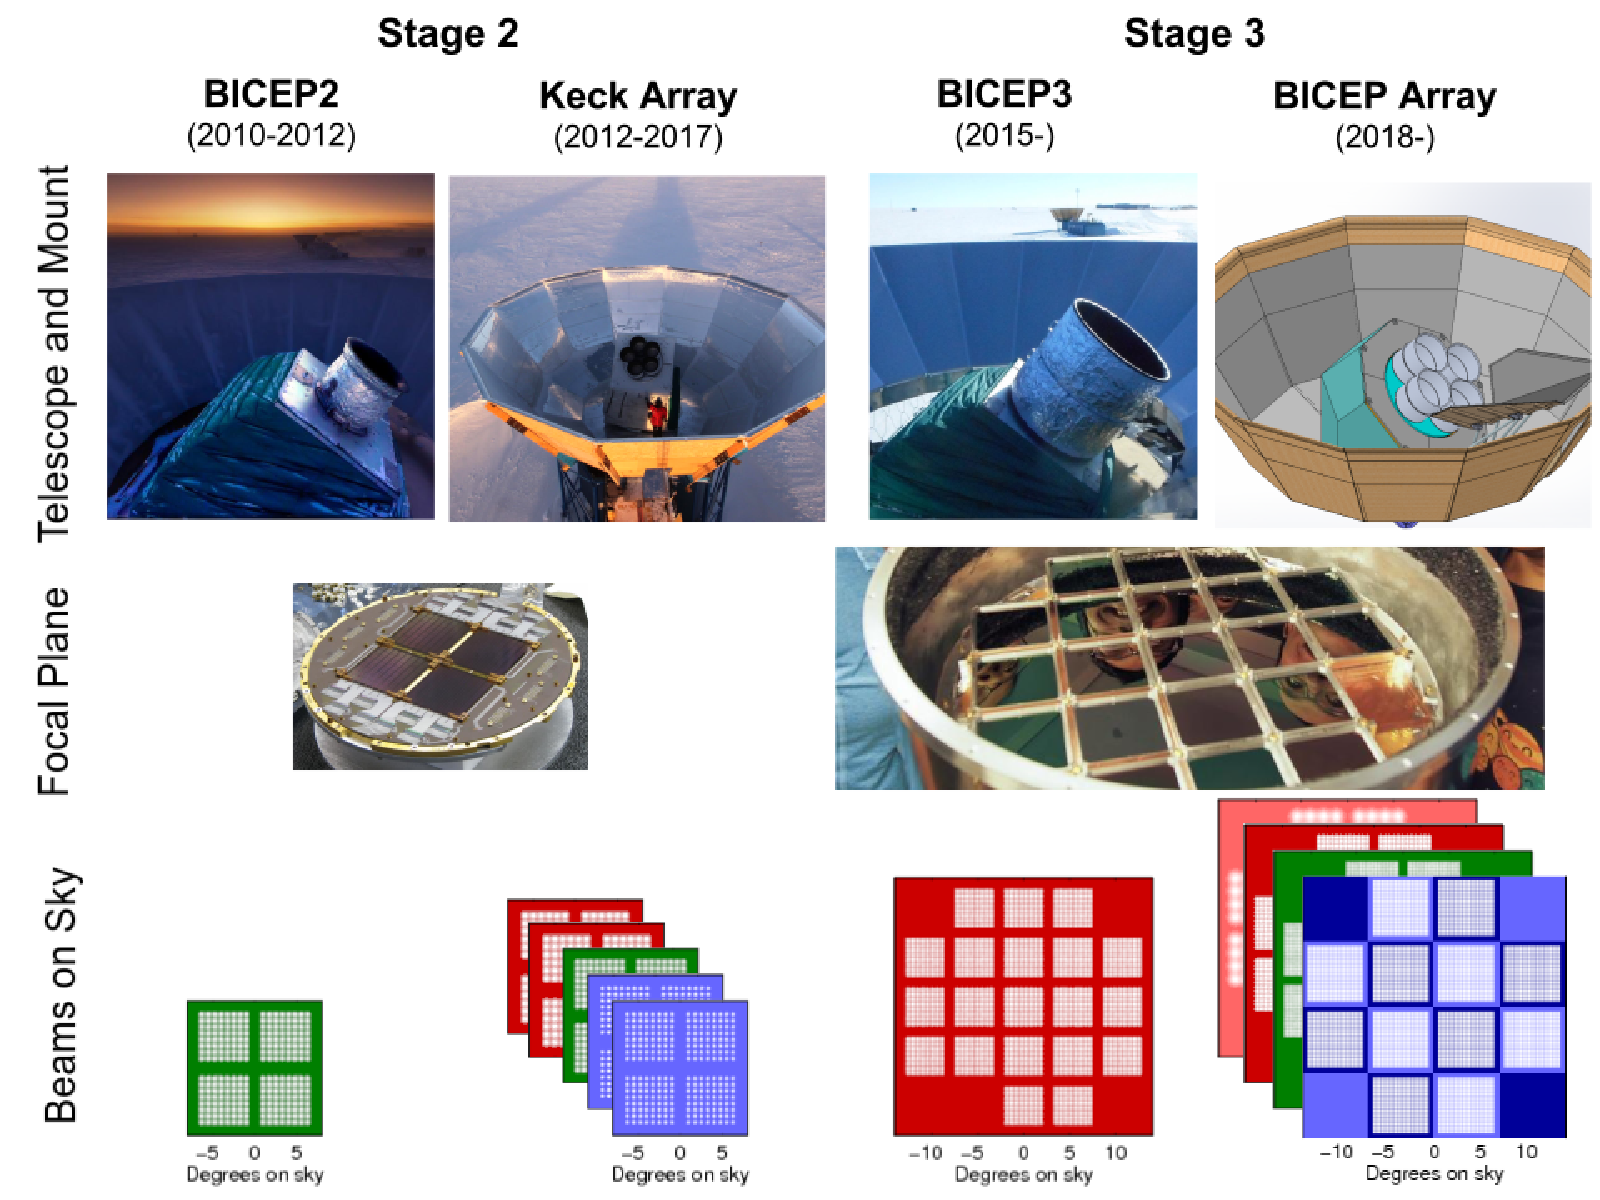
\includegraphics[scale=0.5]{progression.pdf}
	\caption{A graphical representation of the \bk\ experiments from
	\bicep2\ through \biceparray. The middle and bottom rows show the increased focal plane size and density of the \bicep3 style receivers as compared to the \bicep2\ style. Different
	frequencies are represented in the bottom row by individual colors with the lowest frequency
	(30 GHz) visible in light red and the highest (270 GHz) visible in dark
	blue.}
	\label{fig:progression}
\end{figure}

Detection of the inflationary B-mode signal is complicated by the presence of
other B-mode signals. At small angular scales, lensing of curl-free CMB
polarization can convert so called ``E-modes'' into B-modes by relocating
polarized signal across the sky. Other sources of B-mode signal exist in our
own galaxy. Polarized emission from galactic dust and galactic synchrotron
radiation are the two dominant foregrounds in our own galaxy, each
characterized by independent frequency and angular scale relations. Detection
of any primordial B-mode signal requires observations at multiple frequencies
to enable its separation from these foregrounds. 


The \bk\ experiments are a staged series of microwave telescopes that observe
the CMB from the geographic South Pole. Each successive generation of
telescope builds upon the experience gained with the previous while providing
increasingly sensitive data. A graphical progression from \bicep2\ to
\biceparray\ is shown below in Fig.~\ref{fig:progression}. The experiments target degree-scale B-mode
polarization in the CMB which could have been generated by primordial
gravitational waves during the epoch of inflation. Foreground signal exhibits strong frequency dependence which allows these components to be isolated from the IGW
signal by observing the microwave sky across a range of frequencies.
\keckarray\ consists of five \bicep2 style receivers with observations spread
across four frequency bands (95, 150, 220, and 270 GHz). In combination with the \bicep2 data the \keckarray\ has
published the strictest constraint on this signal to date of $r<0.07$
\cite{bk14}. \biceparray\ builds on the success of the \keckarray\ by
deploying four \bicep3 style receivers and expanding observations into two
additional frequency bands at 30, and 40 GHz. Extrapolating from achieved performance,
\biceparray\ is projected to reach $\sigma(r)<0.004$, either detecting the IGW
signal or improving the constraint to $r<0.008$. 



	
\section{Cryostat Design}

\biceparray\ continues the successful design philosophy of
the previous \bk\ receivers. An 80" tall vacuum shell contains two nested
stages with nominal operating temperatures of 50K and 4K which accommodate
optical elements and shield the sub-Kelvin receiver. A cross section of
the cryostat is shown in Fig.~\ref{fig:bavskeck}. The top section of the
vacuum jacket houses the vacuum window and a stack of Zotefoam filters which reduce infrared loading
onto the colder stages. The use of low-conductivity structural supports keeps
the interior stages sufficiently supported while conducting only a small
amount of heat from the room temperature vacuum vessel. These supports are
described in more detail in Sec.~\ref{sec:thermal_architecture}. The
intermediate 50K stage serves as a radiation shield for the interior 4K stage.
The lower $\sim70\%$ of this stage is wrapped with a $0.04''$ thick magnetic
shield composed of Amuneal A4K. The top of this stage additionally
accommodates an alumina filter to further reduce infrared loading onto the
sub-Kelvin receiver. The 4K stage serves as a second radiation shield while
also providing mounting interfaces for two alumina lenses and optical
baffling.

\begin{figure} [hb]
	\begin{center}
		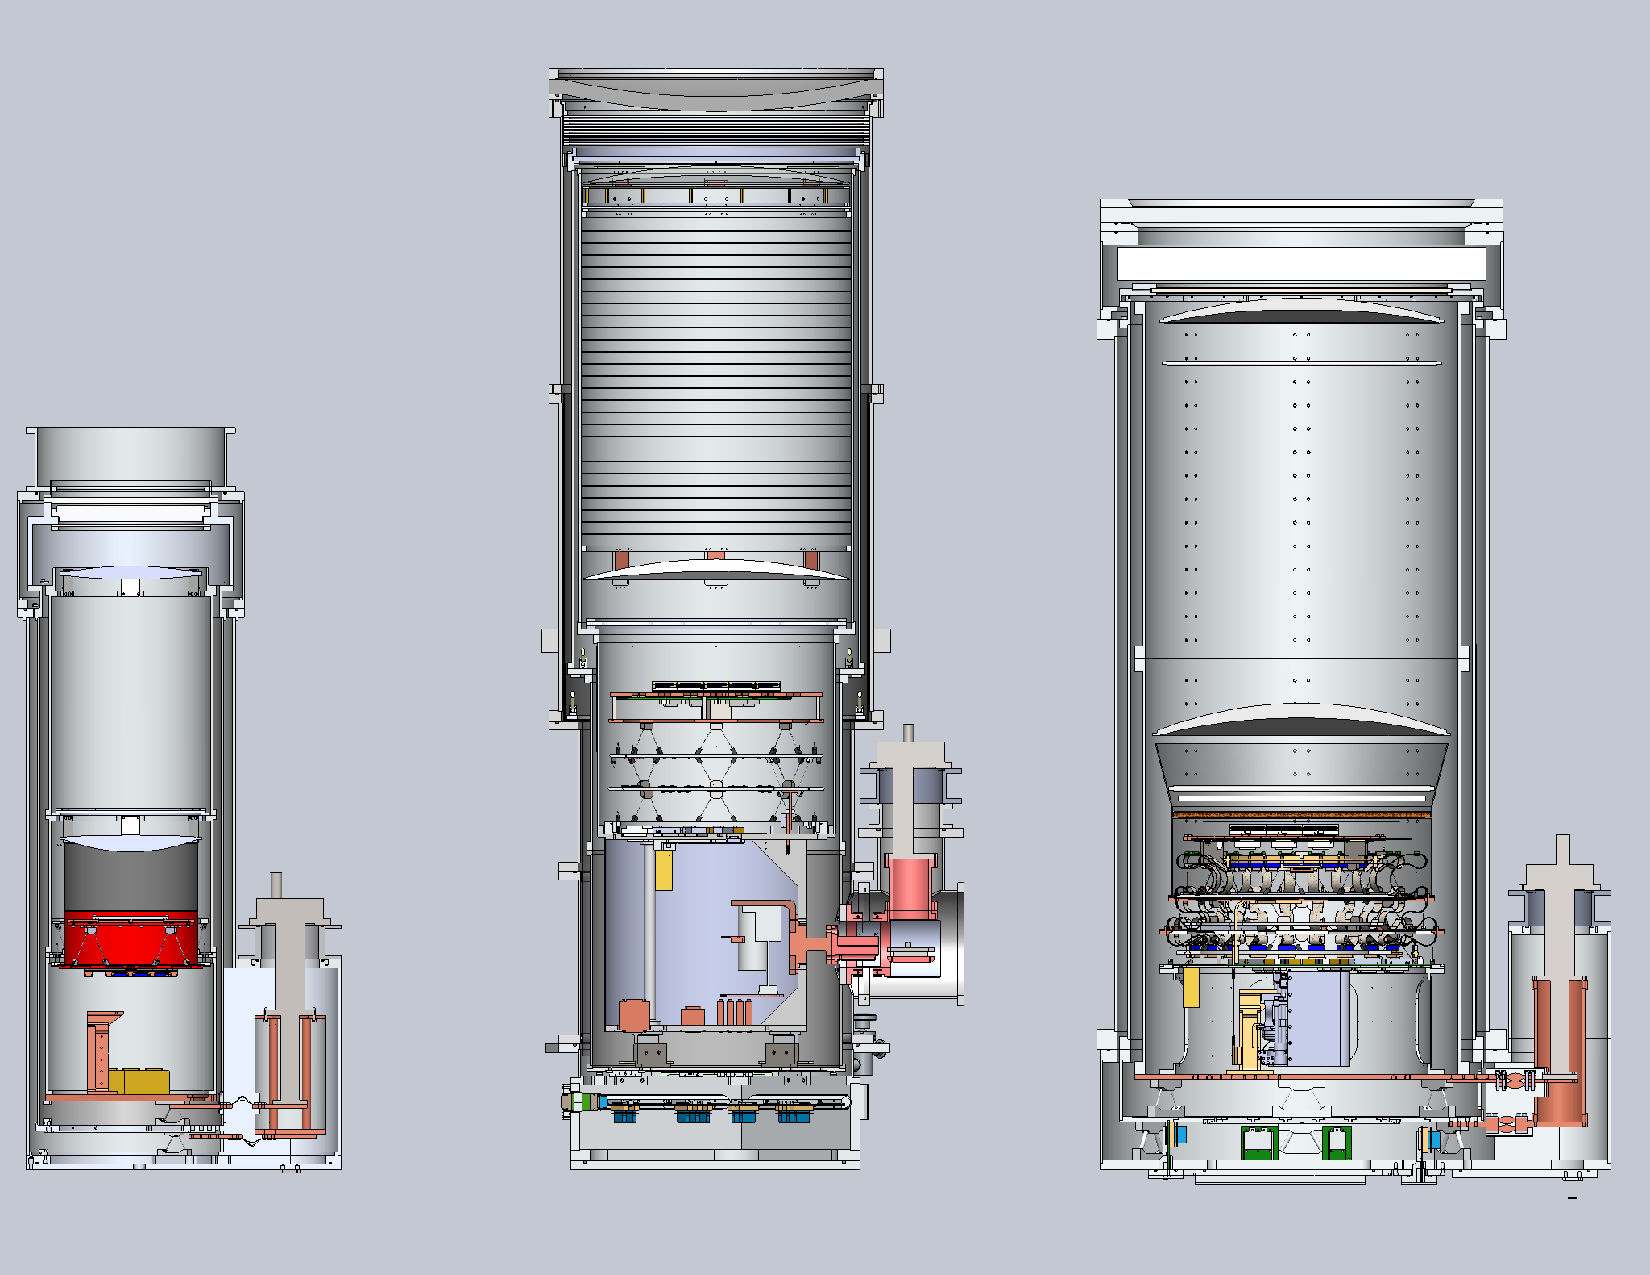
\includegraphics[scale=0.35]{BA_B3_spud.PDF}
	\end{center}
	\caption{A CAD cross section of a single \keckarray\ receiver (left), the
	\bicep3 receiver (middle), and a single
	\biceparray\ receiver (right). The \biceparray\ receivers have double
	the clear aperture and significantly increased focal plane density as
	compared to the \keckarray\ receivers. \biceparray\ also increases the
	width of the cryostat in order to include more optical baffling at the
	lowest frequencies.}
	\label{fig:bavskeck}
\end{figure}







The cryostat design enables ease of access to the focal plane assembly without
disturbing the majority of thermal joints or the back-end cabling. The
cryostat disassembles by lifting off shells successively
from the outside in, leaving a stand-alone base behind which contains the
sub-Kelvin focal plane assembly, readout electronics, and the cooling system as shown in
Fig.~\ref{fig:base}. In this state, the focal plane and detector modules may be
freely accessed for maintenance and other technical activities. Access to the
underside of the focal plane and the readout electronics is provided by
hatches on the bottom side of the vacuum shell and 50K bases. This scheme
significantly reduces the time required for disassembly when accessing the
focal plane and re-assembly afterwards by allowing critical thermal junctions
and difficult part matings to remain undisrupted.

\begin{figure} [h]
	\begin{center}
		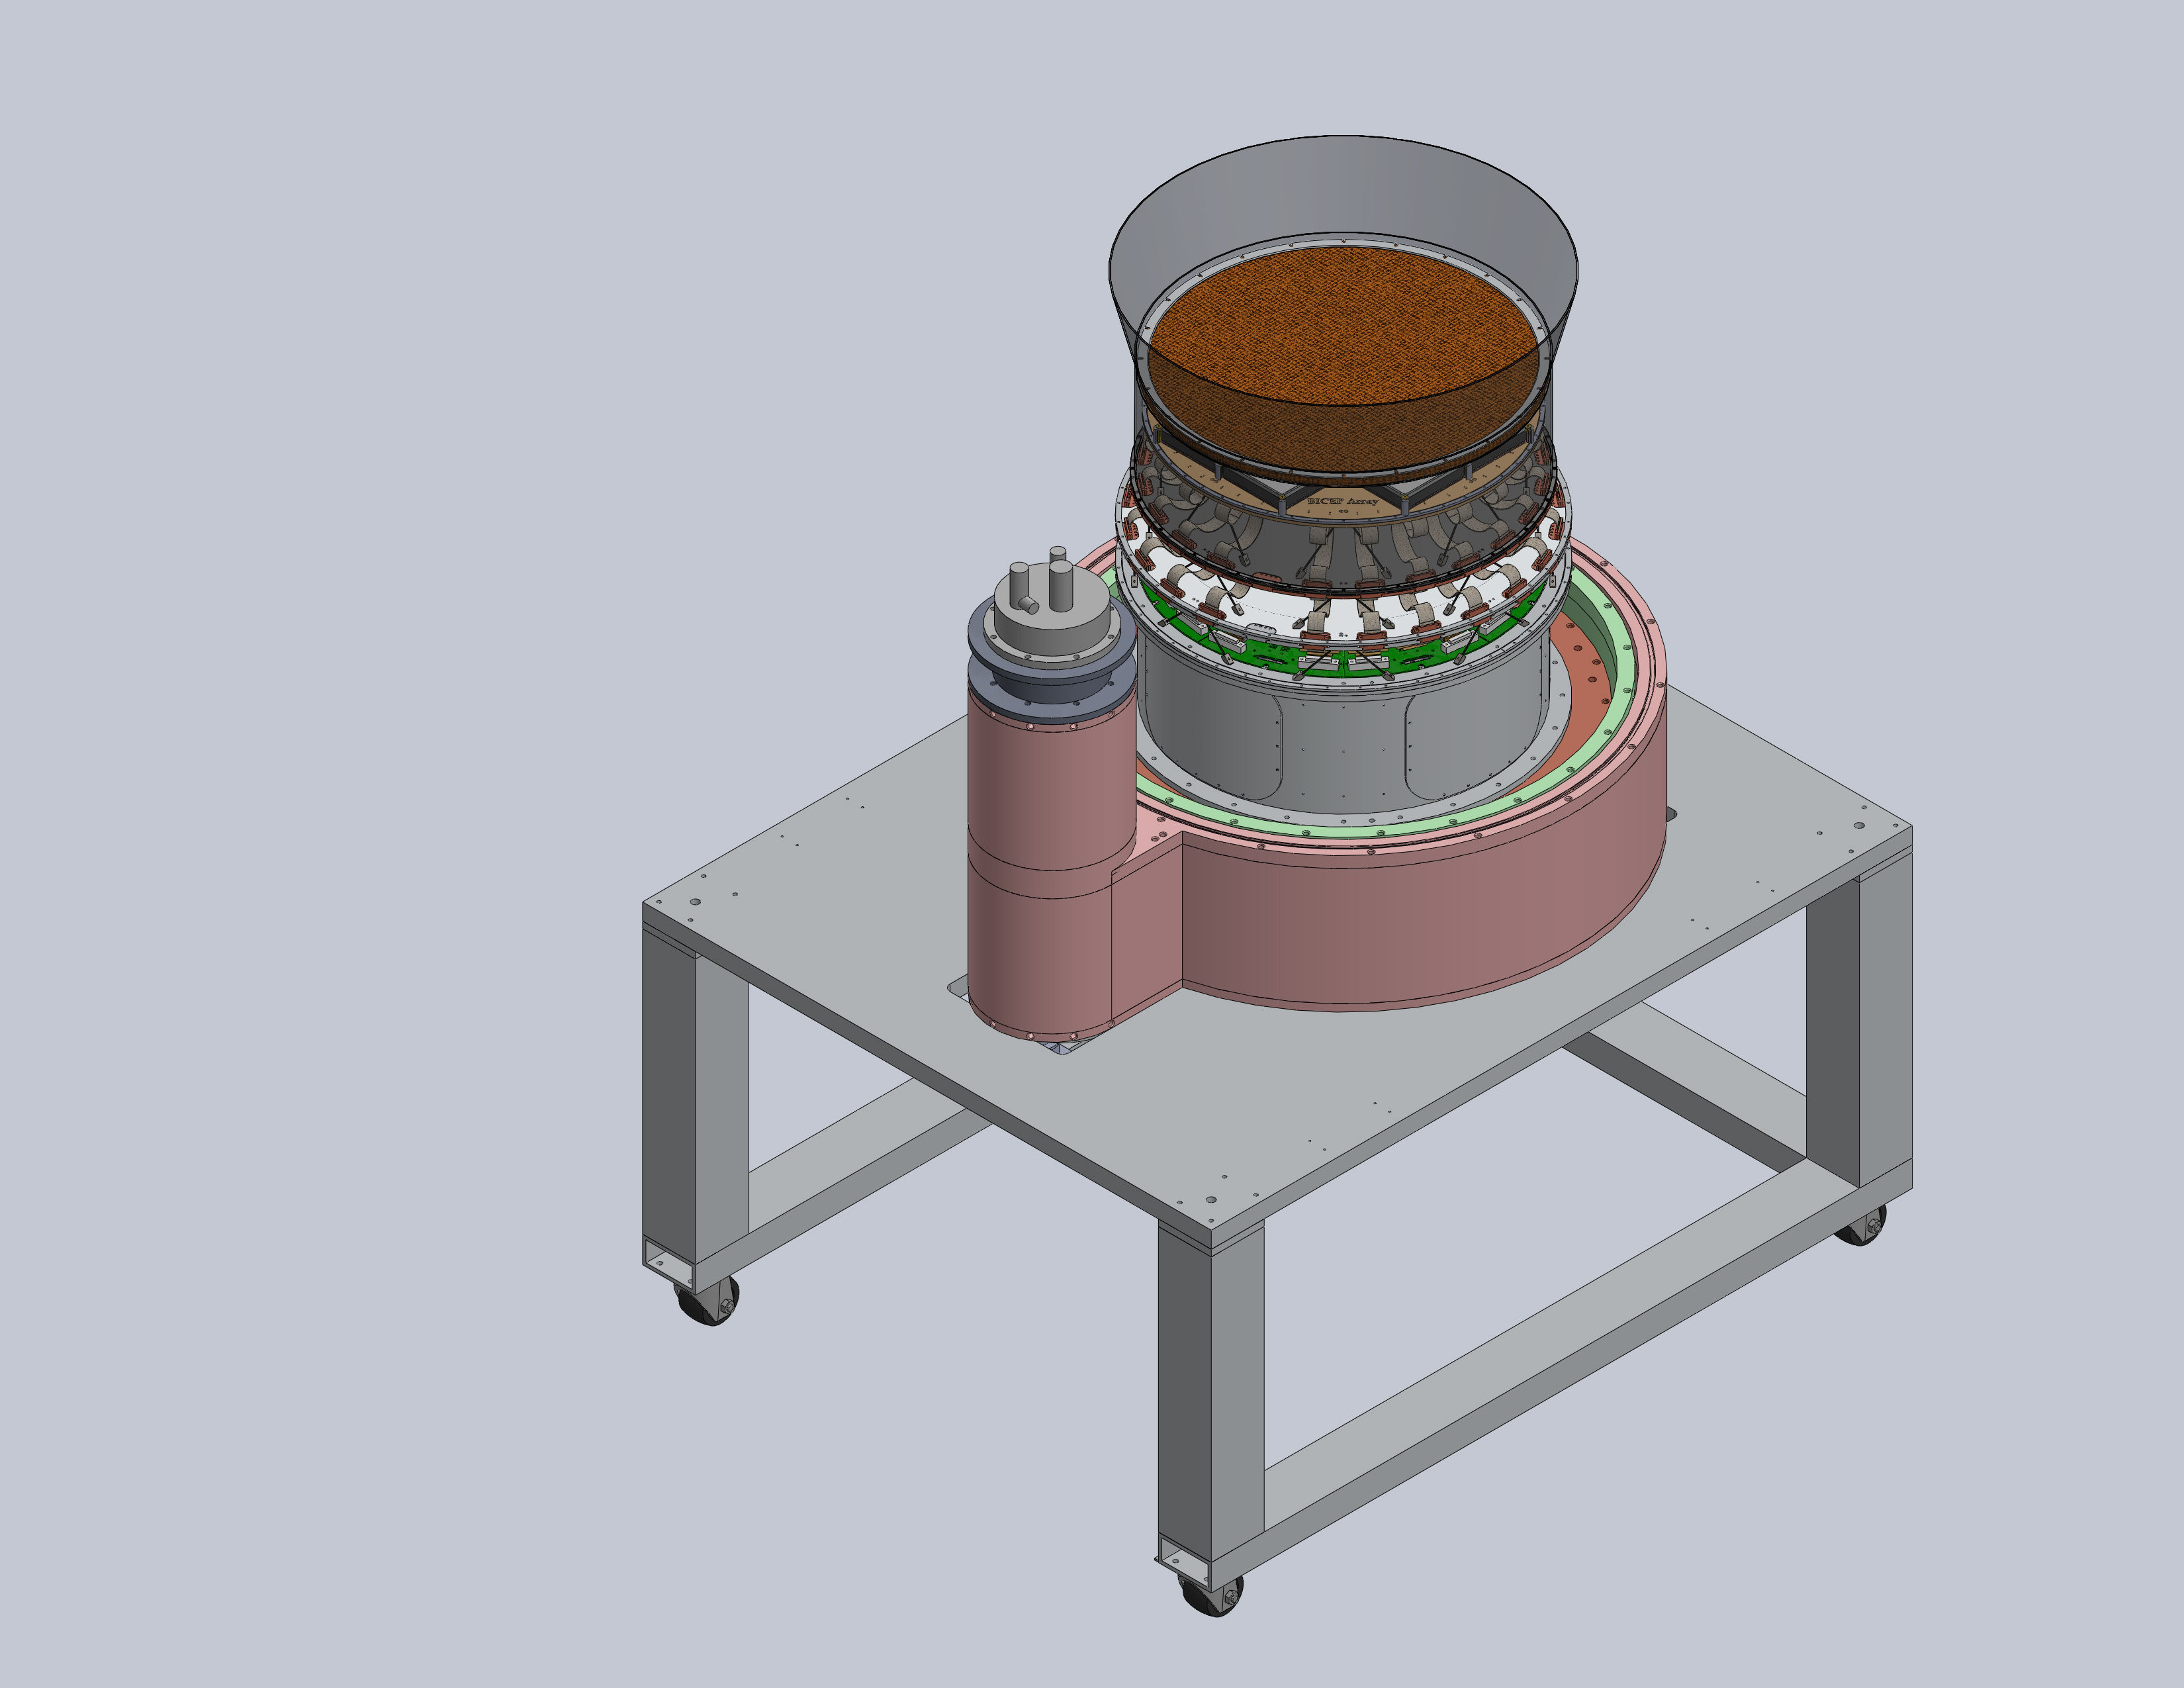
\includegraphics[scale=0.4]{base_on_lowboy.JPG}
	\end{center}
	\caption{A CAD cross section of a single \keckarray\ receiver (left), the
	\bicep3 receiver (middle), and a single
	\biceparray\ receiver (right). The \biceparray\ receivers have double
	the clear aperture and significantly increased focal plane density as
	compared to the \keckarray\ receivers. \biceparray\ also increases the
	width of the cryostat in order to include more optical baffling at the
	lowest frequencies.}
	\label{fig:base}
\end{figure}


\section{Thermal Architecture}
\label{sec:thermal_architecture}

 The 50K and 4K radiation shields are cooled by the first
and second stages respectively of a Cryomech PT415-RM Pulse Tube cooler. This
cryocooler is capable of maintaining a first stage temperature of $<45$K under
a 40W load and a second stage temperature of $<4$K under a
1.5W load. The cooler of these two stages is required to maintain a
sufficiently cold temperature to allow the operation of a three stage helium
sorption fridge which cools the sub-Kelvin receiver. The interior stages must
therefore be well insulated in order to stay within the thermal budget.

\clearpage


The radiation absorbed by the interior stages is reduced by the use of
multi-layer insulation (MLI) wrapped around the outside of the 50K and 4K stages. Where
there is insufficient room for uncompressed insulation, high emissivity
aluminum tape is used on parallel faces to decrease the radiation absorbed by the lower
temperature surface. The radiation shields are additionally attached to higher temperature stages
via a low thermal conductivity support system. The front end of each shell is
constrained by thin Ti-Al-4V straps which are allowed to flex along the axial
direction of the cryostat to absorb differential thermal contraction. At the
back end the 50K and 4K stages are supported by six trusses. Each truss has two high
tensile strength / thermal conductivity rods bonded to aluminum blocks with
Stycast epoxy. We use G10-FR4 for the backend supports between the vacuum
shell and the 50K radiation shield but switch to carbon fiber between the 50K
and 4K shells due to the former's lower thermal conductivity at low
temperatures. Figure~\ref{fig:supports} shows fabricated examples of the
front and back-end supports.

\begin{figure}[t]
	\center
	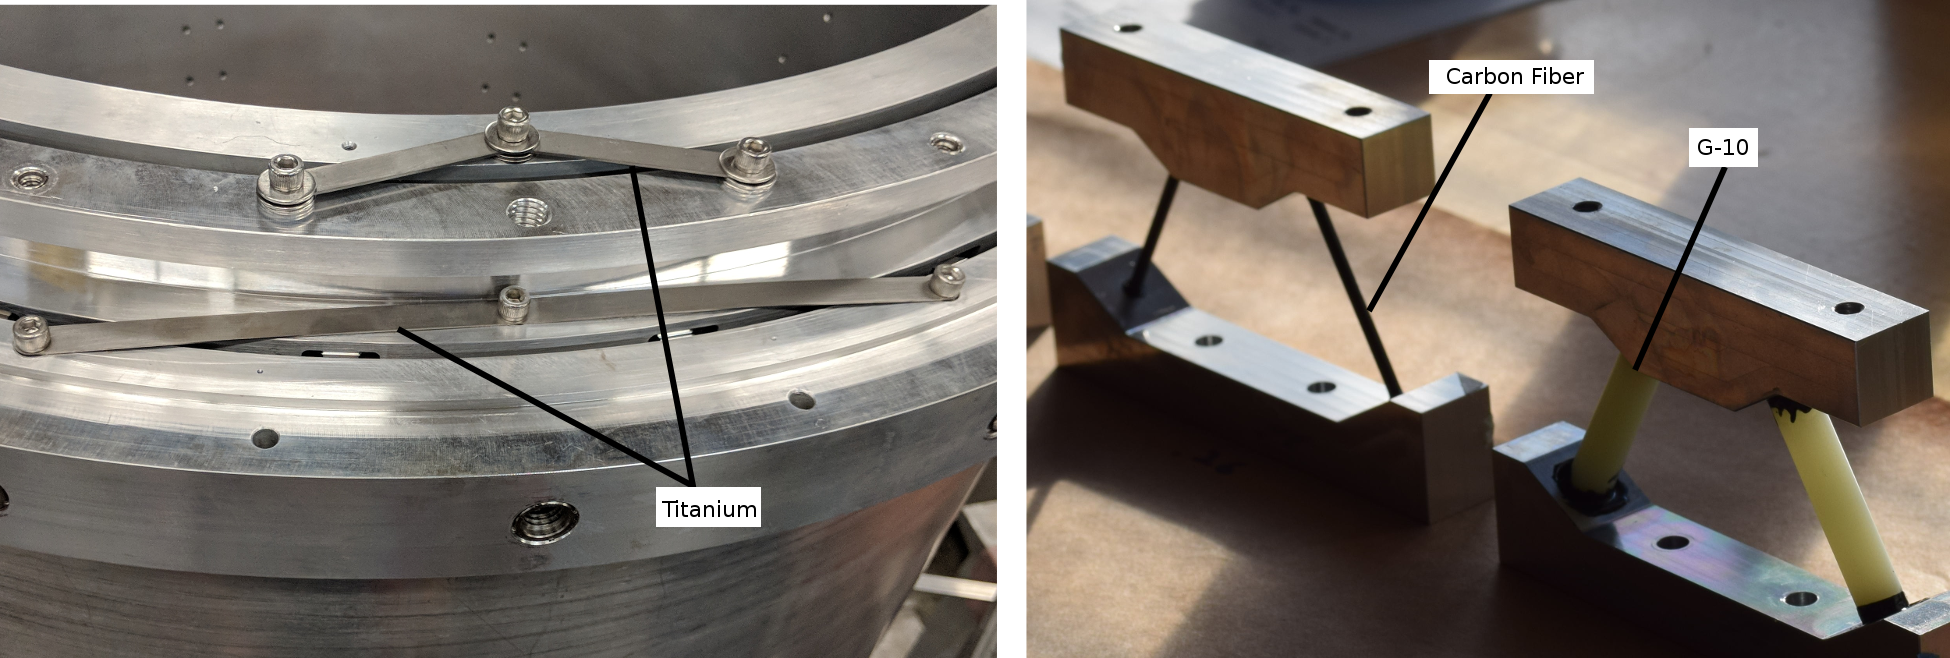
\includegraphics[scale=0.1]{supports.png}
	\caption{\textbf{Left:} The top end titanium supports. These thin strips
	are flexible along the axial direction of the cryostat while rigid enough
	to maintain concentricity of the stages. \textbf{Right:} Example carbon fiber (left) and G10 (right) supports. These
	supports sit at the back end of the cryostat and span the gap between the
	vacuum jacket to 50K stage (G10) and between the 50K and 4K stage (carbon
	fiber). Each rod is held in place with Stycast epoxy.}
	\label{fig:supports}
\end{figure}



In addition to providing radiation shielding and mount points for low
temperature optics, the 50K and 4K stages provide natural heat sinks for the
cryocables that connect the sub-Kelvin electronics to the exterior
room-temperature data acquisition system. By sinking the cryocables to the 50K
stage the conductive loading onto the 50K stage is significantly reduced.
Likewise, the heatsinks on the 4K stage significantly reduce the conductive
loading onto the sub-Kelvin receiver. 



\section{Copper Braid Heat Straps}

The heat straps connecting the pulse tube cooler to the 50K and 4K stages of
the cryostat needs to have large thermal conductance but also be fairly
flexible to suppress vibrations transmitted to the focal plane. \biceparray\ 
uses custom made oxygen-free high thermal conductivity (OFHC) copper
assemblies each composed of multiple straps. As shown
in Fig.~\ref{fig:heatstrap} each heat strap consists of two end blocks
connected by a series of multi-layered braided wire straps. The braided straps
comprise seven layers of OFHC braid pressure fused into a small diameter OFHC
pipe section on either end. The pressure fusing is performed by a hydraulic
press under a load of 20 tons while external constraint is provided by a steel
die. We have been able to achieve thermal conductance of $G=600
\frac{\text{mW}}{\text{K}} \text{  @}4\text{K}$ per strap in laboratory tests.

The heat straps in the \biceparray\ cryostat combine a number of these straps
to achieve high thermal conductance. Two layers of braided straps are
sandwiched around an OFHC plate on both ends. These plates provide mounting
interfaces to the rest of the cryostat and the pulse tube cooler. Stainless
steel plates on the top and bottom sides of this interface allow the use of
1/4'' stainless steel bolts to create a high pressure joint and reduce thermal
contact resistance. Figure~\ref{fig:heatstrap} shows a fully assembled heat
strap assembly that interfaces between the 4K radiation shield and the 2nd
stage of the pulse tube.

\clearpage


\begin{figure}[ht]
\center
\includegraphics[scale=0.4]{heatstraps.png}
\caption{\textbf{Left:} A completed heat strap composed of 6 braided straps. A thin steel plate distributes the force of the bolts and nuts across the surface of the braid ends. \textbf{Right:} A single 7-layer braided strap. This strap is created by inserting layers of OFHC braid into a short OFHC tube and compressing under 20 tons of pressure in a hydraulic press.}
\label{fig:heatstrap}
\end{figure}


\section{Mount and Operations}

The larger size of the \biceparray\ as compared to the \keckarray\ it replaces
requires a larger motorized platform for operation. Designed by Eric Chauvin,
the new \biceparray\ mount uses the same three axis design as the previous
\bk\ experiments which augments the azimuth and elevation axes with
rotation about the boresight of the array. A
cross section of the new mount assembly is shown below in Fig.~\ref{fig:bamount}.
As with previous \bk\ experiments, the cryostats
are enclosed within an accordion-like environmental shield which co-rotates in
azimuth and flexes as the mount tips down in elevation. A separate central
plate provides a mounting interface for four optical baffles---one per
receiver---and co-rotates with the receivers about the array boresight.


\begin{figure} [hb]
	\begin{center}
		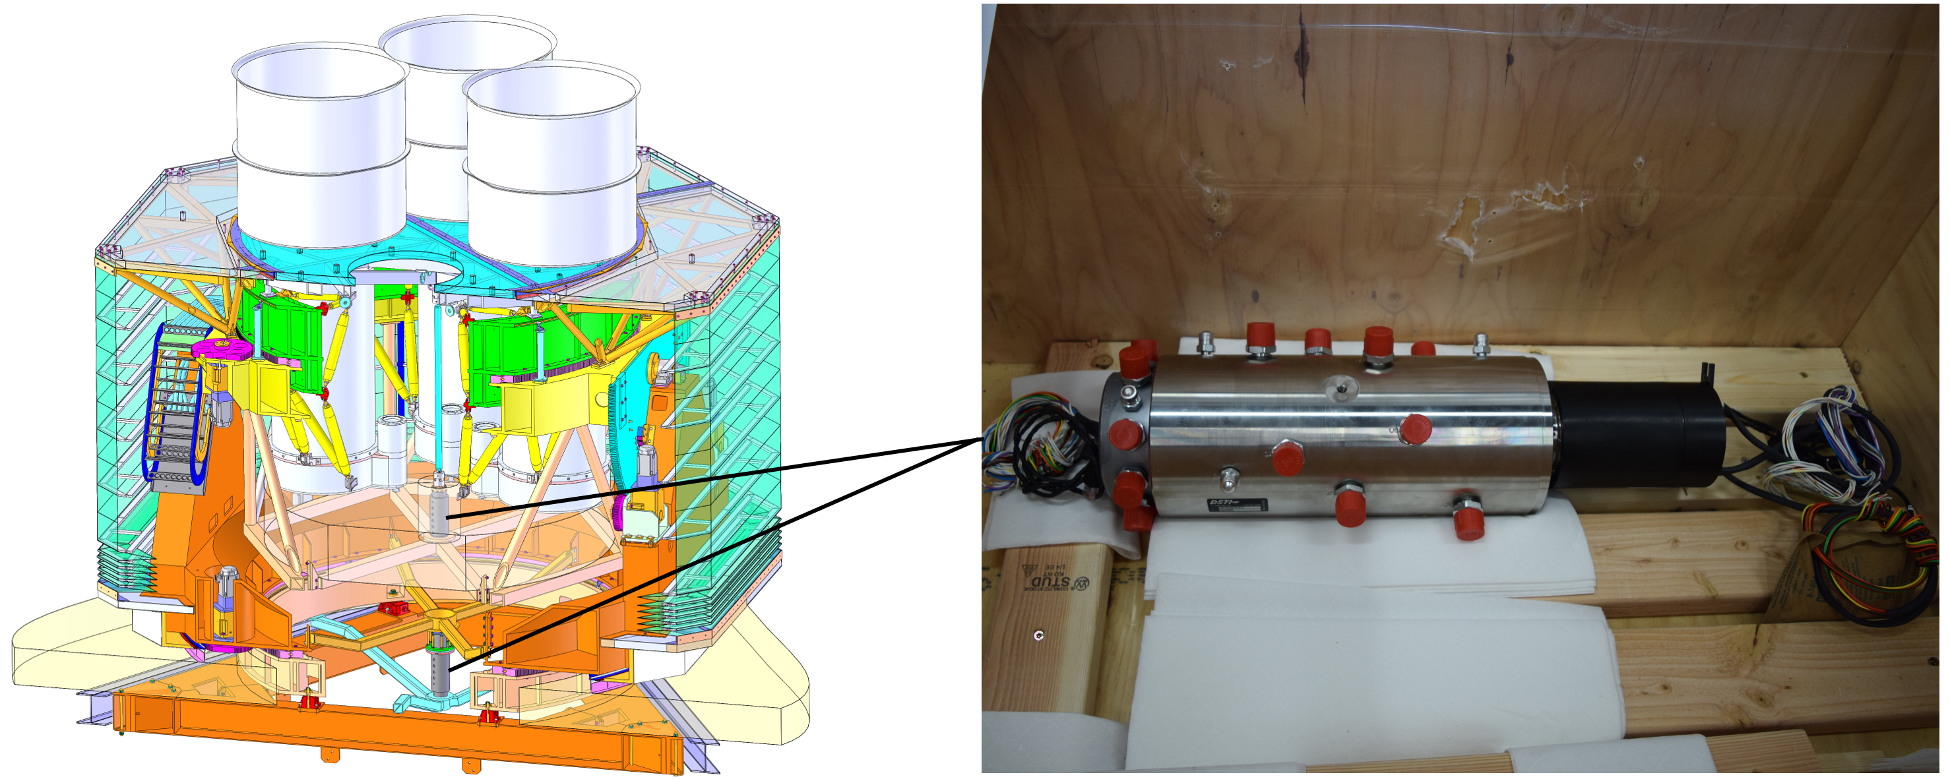
\includegraphics[scale=0.65]{mount.png}
	\end{center}
	\caption{\textbf{Right:} A CAD rendering of the new \biceparray. The surrounding
	accordion-like environmental shield is shown in teal while the two rotary
	unions are depicted in gray and can be seen along the central axis of the
	mount. The large cylinders on the top side of the mount assembly are the co-moving optical baffles that help to reduce sidelobe response. \textbf{Left:} One of the rotary unions from DSTI. Red caps
	denote the locations of helium lines while the electrical and data connections
	can be seen exiting either end of the union.}
	\label{fig:bamount}
\end{figure}

\clearpage

The \biceparray\ mount includes two separate rotary unions which allow
continuous rotation about the azimuth and deck axes without the need for a
cable wrap. These rotary unions were designed at DSTI and each contain 10
helium channels. Eight of these connect the pulse tubes and their compressors
while two channels serve as pressure guards. An additional nitrogen channel
provides a pressurized environment on the backside of thin membrane
structures which shield the receivers' vacuum windows from the Antarctic winter.
Inclusion of slip rings at both ends of the union additionally provide data and power
connections to electronics fixed to the same structure as the cryostats. These rotary
unions allow the helium compressors---required to operate the
pulse tube coolers---to sit well below the mount structure in the
stationary tower. Helium lines route upwards into the lower fixed half of the first
rotary union and then out through the upper half which rotates in azimuth
along with the receivers. The hoses from the upper half are then routed through a
short cable chain that provides flexure when rotating in elevation. The
second rotary union is then similarly connected with the free section rotating
about the array boresight.



\biceparray\ will consist of four receivers observing in 6 frequency bands.
Two receivers will continue to observe in the 95 and 150 GHz bands where the
\bk\ maps are deepest and where combined foreground
signal is at a minimum. These will be augmented by two dual-band receivers at
30/40 GHz and 220/270 GHz with the two frequencies interleaved in a
checkerboard pattern. With the increased sensitivity at 95 and 150 GHz these
two additional receivers will be required to push constraints on polarized
emission from galactic synchrotron and dust further than the currently available data.
The 30/40 GHz receiver will extend the observations into two
new bands at which the synchrotron foreground is expected to dominate. The
\keckarray\ is already observing in the 220 and 270 GHz bands.  However with
significantly increased throughput and a detector count of over 9 times the
entire \keckarray, the dual band 220/270 GHz \biceparray\ receiver will rapidly
eclipse current sensitivity. In only a few days of observation,
this receiver will surpass the dust sensitivity of the \planck\ 353 GHz data in
the \bk\ field. 

The observing power of \biceparray\ will be concentrated on the same $\sim400
\text{ deg}^2$ patch of sky as the existing \bk\ data. By directly
observing cosmological foregrounds with the new dual band receivers in the
patch at which the \bk\ data is already the deepest we will be able to
directly constrain these foregrounds in our own patch of sky, significantly
reducing the effect of any spatial variation in the foregrounds' spectral
energy distribution. Increasing foreground constraints will be complemented by
simultaneously increasing sensitivity to $r$ with the single band receivers. Figure~\ref{fig:projections} shows the sensitivity projections for \biceparray. All projections are based on achieved sensitivity and as such, build in real world inefficiencies such as detector yield, weather, and other factors which decrease overall sensitivity. By the end of the program, \biceparray\ is projected to constrain $r<0.008$, $\sigma (r)<0.004$.


\begin{figure}[hb]
\center
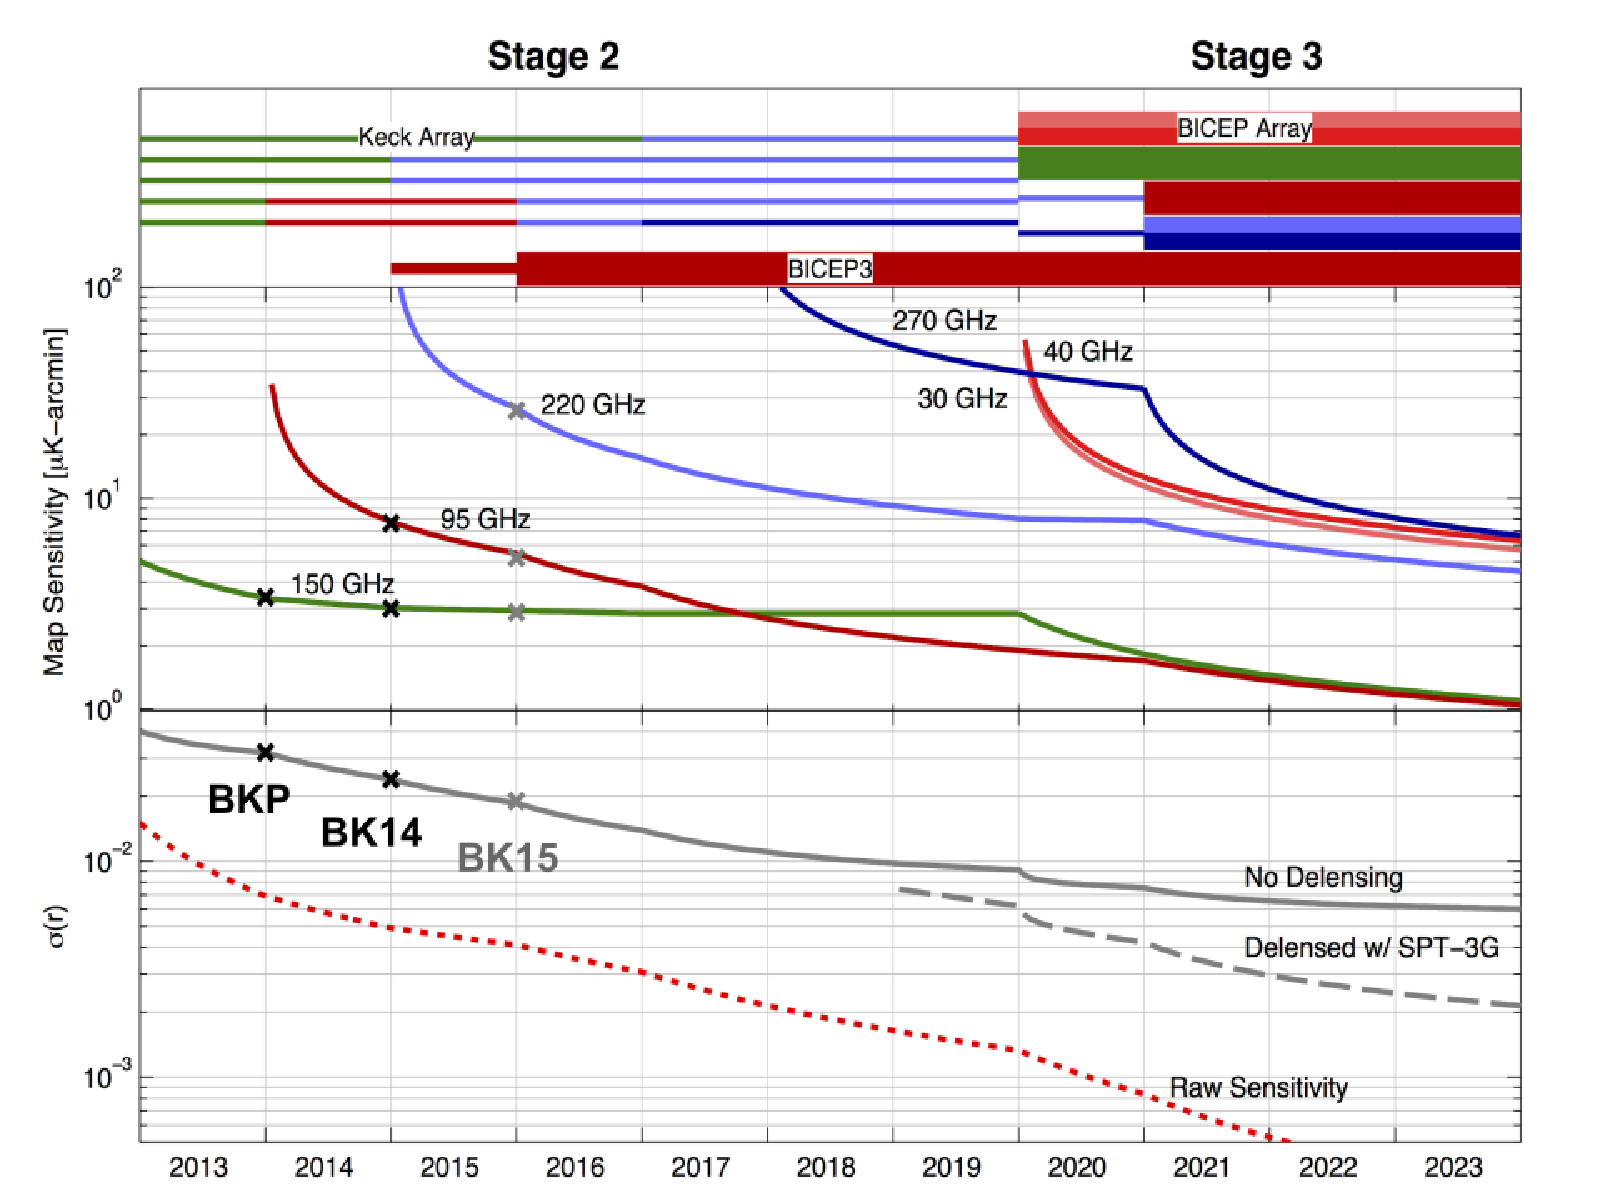
\includegraphics[scale=0.4]{projections.pdf}
\caption{Achieved and projected sensitivity for the current and planned \bk\ program. \textbf{Top:} A representation of receiver throughput at different frequencies. \textbf{Middle:} Achieved and projected map depth at various frequencies as a function of time. Black X's mark achieved sensitivities in the BKP\cite{bkp} and BK14\cite{bk14} papers while gray X's show achieved sensitivity in the upcoming BK15 paper. \textbf{Bottom:} Sensitivity to $r$, marginalizing over the seven parameter foreground model as described in BK14. Raw sensitivity in the absence of foregrounds is also shown.}
\label{fig:projections}
\end{figure}









% References
\bibliography{report} % bibliography data in report.bib
\bibliographystyle{spiebib} % makes bibtex use spiebib.bst

\end{document} 
